\documentclass[11pt]{article}
\usepackage[margin=0.75in]{geometry}            % See geometry.pdf to learn the layout options. There are lots.
\geometry{letterpaper}                                  % ... or a4paper or a5paper or ... 
%\geometry{landscape}                           % Activate for rotated page geometry
%\usepackage[parfill]{parskip}                  % Activate to begin paragraphs with an empty line rather than an indent
\usepackage{graphicx}                           % Use pdf, png, jpg, or eps§ with pdflatex; use eps in DVI mode
                                                                % TeX will automatically convert eps --> pdf in pdflatex                
\usepackage{amssymb}
\usepackage{upquote}
\usepackage [autostyle, english = american]{csquotes}
\MakeOuterQuote{"}
\usepackage{multirow}
\usepackage{colortbl}
\definecolor{kugray5}{RGB}{224,224,224}

%-----------------------------------------------------------------------------
% Special-purpose color definitions (dark enough to print OK in black and white)
\usepackage{color}
% A few colors to replace the defaults for certain link types
\definecolor{orange}{cmyk}{0,0.4,0.8,0.2}
\definecolor{darkorange}{rgb}{.71,0.21,0.01}
\definecolor{darkgreen}{rgb}{.12,.54,.11}
%-----------------------------------------------------------------------------
% The hyperref package gives us a pdf with properly built
% internal navigation ('pdf bookmarks' for the table of contents,
% internal cross-reference links, web links for URLs, etc.)
\usepackage{hyperref}
\hypersetup{pdftex, % needed for pdflatex
  breaklinks=true, % so long urls are correctly broken across lines
  colorlinks=true,
  urlcolor=blue,
  linkcolor=darkorange,
  citecolor=darkgreen,
}


\title{Forecasting Price Changes in High Frequency Trading Data\\
  Stat 222, Spring 2016}

\author{
  Sici Huang, Alanna Iverson, Jamie Palumbo\\
  \texttt{https://github.com/sicihuang/Finance-Project}
}


\begin{document}
\maketitle

\section{Introduction}

It has always been in the interest of the investor to predict price movements in order to gain insights into trends and to profit from the stock market. With the rise of high frequency trading, financial service agencies have become interested in utilizing machine learning models for prediction. Our report closely follows the methodology in Kercheval and Zhang \cite{ky} which builds random forest and SVM classifiers to forecast price changes using the limit order book. The following report explains our data preprocessing strategies, the model fitting process, and our model assessment along with derived trading strategies and the associated profits. 



\section{Data Preprocessing}

Finding the right features to train our models on was essential to this project. We included the same features for both the random forests and the support vector machines, though some features were scaled differently between the two. Our features were based heavily on the Kercheval and Zhang paper and improved through trial and error. The first decision we needed to make was how to deal with the multiple values per time in the LOB data. To handle this, we examined the definition of "best bid" and "best ask." Since the "best bid" is the highest bid, we chose the maximum of the bids for each row of the data as the bid value. Similarly, since the minimum ask is the "best ask" price per row, we chose the minimum value as the ask price for each time $t$. Once we had a bid and ask price for each time point, we began constructing features on top of these values that might be helpful in training our models. Since we also wanted volume information, we consolidated the volume data per row by taking the mean of each row and saving the information in a new feature for each time point for both ask and bid volumes.\\
\\
The next features we created were rolling means for the best bid and best ask prices with a window of 10. This calculates the average of the 10 values above and below each row as a new feature so that we can determine whether the average is increasing or decreasing over time. This is similar to $v4$ in the Kercheval and Zhang paper. Our next feature was to simply use the maximum bid and minimum ask features from above in order to calculate the mid price for every time $t$. An analogous process was used to calculate the rolling means of the average ask and bid volumes per time $t$. Again using the maximum bid and minimum ask features from previous calculations, we calculated the price difference between the two by subtracting the maximum bid from the minimum ask. A similar calculation was made for each row of the data for the average volumes.\\
\\
SVMs tend to prefer data that is similarly scaled across features so that no one feature dominates others. Conversely, random forests tend to perform well regardless. Therefore, we created a function that calculates data on the regular and log scales where appropriate. For example, since the difference in price is typically on the order of pennies, we do not log scale this feature when training our random forests. However, since maximum bid and minimum ask prices are over \$500, we log scale this feature before fitting the SVMs. \\
\\
Initially, our training data also included features that were based on $v8$ in Kercheval and Zhang. We created an indicator variable that was a one if the average bid volume or ask volume increased from time $t$ to time $\Delta t$. However, after increasing these features and evaluating performance of our models on the validation set, we determined that they did not increase performance and decided to remove them.\\
\\
In summary, we trained our random forest models on a feature set that included 13 variables: the maximum bid price, the rolling mean of the maximum bid price, the difference in bid price between each $\Delta t$ interval, the minimum ask price, the rolling mean of the minimum ask price, the difference in ask price between each $\Delta t$ interval, the average of the two prices, the average bid and ask volumes, the rolling means of the bid and ask volumes, the difference between minimum ask and maximum bid, and the difference in ask and bid volumes for each time $t$. Our SVMs were trained on analogous datasets that took the log of each variable except the difference in ask and bid prices between each $\Delta t$ interval and the difference between minimum ask and maximum bid.\\
\\
In order to study mid price movement, we created three columns with a one-vs-all strategy in mind to handle the prediction of more than two classes. In other words, in order to evaluate whether the mid price movement between $t$ and $\Delta t$ was upward, stationary, or downward, each direction had its own column. If the movement was upward, then that $t$ value was assigned a one. A zero was assigned for every other movement type. The same procedure was followed in order to determine whether spread crossing movement was upward, stationary, or downward. The idea is that we will train six random forests and six SVMs to predict the six movement types described above in order to interpret our model.\\
\\
Finally, we split the data set into a training set, validation set, and test set. In order to do this, we used a logical method to subset the data based on the Time column. Data that was gathered before 10:30 AM was used as the training data. Data gathered between 10:30 AM and 11:00 AM was used as the validation set, and data gathered after 11:00 AM was used as the test set. 



\section{Model Fitting}
Once we had features sets we believed satisfied the requirements of this project, we began fitting the six decision trees and six SVMs. With both of these machine learning algorithms, the choice of hyperparameters can drastically change performance. For decision trees, these hyperparameters are the number of trees in the forest and the maximum depth of the trees used. For SVMs, the hyperparameters are the C and gamma values chosen. In both cases, we decided to use average cross-validation scores \big(the scikit learn function cross\_val\_score with cv $=$ 5\big) with the training data in order to choose the best values. Once we had a handful of hyperparameter values that produced the most accurate predictions on the cross-validated training data, we used the validation set in order to choose the final set of parameters. The hyperparameter values that gave the highest accuracy on the validation set after being trained on the training set were chosen.\\
\\
Our final task in this section was to determine the best $\Delta t$ value to make our predictions useful but not too computationally expensive. In order to do this we fit each of the algorithms with the process described above three times with different $\Delta t$ values. We then determined the highest accuracy of each of the models per $\Delta t$ value and chose the $\Delta t$ that had the highest validation set accuracy most often. However, before we could do this, we needed to narrow down three choices of $\Delta t$. After some exploratory analysis, we found that $\Delta t$ values of less than 20 would simply predict every mid price movement as stationary -- not very helpful. Because of this, we chose to fit the models with three $\Delta t$ values that allowed us to make non-stationary predictions without becoming too difficult, namely $\Delta t$ values of 20, 25, and 30. We discovered that the $\Delta t$ of 30 gave us the highest accuracy on the validation set, our way of choosing the "best" value. With this $\Delta t$, we fit the models with the most accurate hyperparameters in order to make our final predictions on the test set. The results of these predictions are presented in the next section on model assessment.

\begin{figure}
  \centering
  
  \begin{tabular}{ | c | c | c | }
    \hline
    $\Delta t = 30$ & RF Validation Set Accuracy & SVM Validation Set Accuracy  \\ \hline
    
    Upward Mid & \begin{tabular}{@{}c@{}}0.5718638902996445 \\ $trees=110$, $depth=2$ \end{tabular} & \begin{tabular}{@{}c@{}}0.5678009141696293 \\ $C=2^{10}$, $gamma=2^{10}$ \end{tabular}  \\ \hline
    
    Stationary Mid & \begin{tabular}{@{}c@{}}0.8781107160995429 \\ $trees=310$, $depth=2$ \end{tabular} & \begin{tabular}{@{}c@{}}0.8781107160995429 \\ $C=2^{10}$, $gamma=2^{10}$ \end{tabular}  \\ \hline
    
    Downward Mid & \begin{tabular}{@{}c@{}}0.5865921787709497 \\ $trees=310$, $depth=2$ \end{tabular} & \begin{tabular}{@{}c@{}}0.5545962417470798 \\ $C=2^{10}$, $gamma=2^{10}$ \end{tabular}  \\ \hline
    
    Upward Cross & \begin{tabular}{@{}c@{}}0.9954291518537328 \\ $trees=10$, $depth=16$ \end{tabular} & \begin{tabular}{@{}c@{}}0.9954291518537328 \\ $C=2^{10}$, $gamma=2^{10}$ \end{tabular}  \\ \hline
    
    Stationary Cross & \begin{tabular}{@{}c@{}}0.9873031995937024 \\ $trees=310$, $depth=2$ \end{tabular} & \begin{tabular}{@{}c@{}}0.9873031995937024 \\ $C=2^{10}$, $gamma=2^{10}$ \end{tabular}  \\ \hline
    
    Downward Cross & \begin{tabular}{@{}c@{}}0.9923819197562215 \\ $trees=310$, $depth=2$ \end{tabular} & \begin{tabular}{@{}c@{}}0.9923819197562215 \\ $C=2^{10}$, $gamma=2^{10}$ \end{tabular}  \\ \hline
    
  \end{tabular}  
  \caption{Parameter Selection}
  \label{fig:parameter}
\end{figure}

\section{Model Assessment}
We can see from Figures 2 and 3 that the random forests resulted in better predictions of mid price movement, but the models were identical in predicting test set spread crossings. This is due to the fact that the optimal $\Delta t$ value of 30 for predicting mid price creates models that predict almost exclusively stationary values on the test set for spread crossings, even though this was not the case on the validation set. So even though we followed a rigorous process to train the models and use the validation set, it appears that they did not perform to our expectations on the test set for spread crossings. Since it was unclear in the guidelines for the project whether mid price and spread crossing models could have different $\Delta t$ values, we chose to stick with one to be safe. In the future, it might be useful to choose a larger $\Delta t$ value for predicting spread crossings rather than predicting mid price movement based on our results.
\begin{figure}
  \centering
    \includegraphics[width=0.8\textwidth]{modelaccuracy}
  \caption{Model Accuracies}
  \label{fig:find3}
\end{figure}


\begin{figure}
  \centering
  \begin{tabular}{|c|l|l|l|l|l|}
    \hline
    \multicolumn{2}{|>{}c|}{$\Delta t = 30$} & \multicolumn{2}{c|}{RF Test Set Metrics} & \multicolumn{2}{c|}{SVM Test Set Metrics} \\
    \cline{3-6}
    \multicolumn{2}{|>{}c|}{} & \multicolumn{1}{p{2cm}|}{Class 0} & \multicolumn{1}{p{2cm}|}{Class 1} & \multicolumn{1}{p{2cm}|}{Class 0} & \multicolumn{1}{p{2cm}|}{Class 1}\\
    \hline
    
    
    \multirow{3}{*}{Upward Mid} &
    Precision & 59.47\% & 65.63\% & 59.22\% & 0\%\\
    \cline{2-6} &
    Recall & 99.44\% & 1.55\% & 99.99\% & 0\%\\
    \cline{2-6} &
    F1 Score & 74.43\% & 3.03\% & 74.39\% & 0\%\\
    \hline
    
    
    \multirow{3}{*}{Stationary Mid} &
    Precision & 86.47\% & 0\% & 86.47\% & 0\%\\
    \cline{2-6} &
    Recall & 100\% & 0\% & 100\% & 0\%\\
    \cline{2-6} &
    F1 Score & 92.74\% & 0\% & 92.74\% & 0\%\\
    \hline
    
    
    \multirow{3}{*}{Downward Mid} &
    Precision&58.18\%&56.38\%&54.33\%&100\%\\
    \cline{2-6}&
    Recall&78.77\%&32.64\%&100\%&0.01\%\\
    \cline{2-6}&
    F1 Score&69.23\%&41.34\%&70.41\%&0.01\%\\
    \hline
    
    
    \multirow{3}{*}{Upward Cross} &
    Precision & 99.43\% & 0\% & 99.43\% & 0\%\\
    \cline{2-6} &
    Recall & 99.99\% & 0\% & 100\% & 0\%\\
    \cline{2-6} &
    F1 Score & 99.71\% & 0\% & 99.71\% & 0\%\\
    \hline
    
    
    \multirow{3}{*}{Stationary Cross} &    
    Precision & 0\% & 98.92\% & 0\% & 98.92\%\\
    \cline{2-6} &
    Recall & 0\% & 100\% & 0\% & 100\%\\
    \cline{2-6} &
    F1 Score & 0\% & 99.45\% & 0\% & 99.45\%\\
    \hline
    
    
    \multirow{3}{*}{Downward Cross} &    
    Precision & 99.51\% & 100\% & 99.51\% & 100\%\\
    \cline{2-6} &
    Recall & 100\% & 0\% & 100\% & 0\%\\
    \cline{2-6} &
    F1 Score & 99.76\% & 0\% & 99.76\% & 0\%\\
    \hline
    
  \end{tabular}
  \caption{Model Assessment Metrics}
  \label{fig:metrics}
\end{figure}



\section{Interpretations}
We determined several simple summary statistics of the LOB that are useful for predicting price movements. If bid price or ask price increases, then there is likely an increase in mid price which indicates there might be an upward spread crossing. If spread increases, then the market stabilizes, meaning it is highly likely that there will not be a spread cross.\\ 
\\
In our final step, we fit a logistic regression in order to compare the results with the previous machine learning approaches. As mentioned previously, random forest performed the best on the test set compared to SVM. In terms of prediction accuracy, random forest performed better than the logistic regression as well but not by much. After taking the log of each of the coefficient values, we can then interpret the odds ratio for each of the models. The odds of a stationary spread crossing are 340.97 and 4.21 times greater if there is a marginal increase of one for spread and ask price, respectively. Upward mid movement also experiences increased odds for similar features. The odds ratios of a downward spread crossing are 0.0096 and 0.32 if there is a marginal increase of one for the spread and ask price, respectively. Similarly, downward mid movement and upward spread crossing experience decreased odds as well. 

\begin{figure}
  \centering
  
  \begin{tabular}{ | l | c | c | c | }
    \hline
     \multicolumn{1}{|>{}c|}{Predictors} & Upward Mid & Stationary Mid & Downward Mid \\ \hline
    
    Log Max Bid & 1.011980 & 0.919934 & 0.988159 \\ \hline
    
   	Log Cum Avg Max Bid & 0.988123 & 0.921812 & 1.000053 \\ \hline
    
    Bid Price & 4.404100 & 1.245018 & 0.219595 \\ \hline
    
    Log Min Ask & 1.012088 & 0.919994 & 0.988053 \\ \hline
    
    Log Cum Avg Min Ask & 0.989856 & 0.920955 &  0.999557 \\ \hline
    
    Ask Price & 3.292218 & 1.557054 & 0.246598 \\ \hline
    
    Log Mid Price & 1.012034 & 0.919963 & 	0.988106 \\ \hline
    
    Log Avg Bid Vol & 0.720115 & 1.636029 & 	1.128983 \\ \hline
    
    Log Cum Avg Bid Vol & 1.145650 & 0.817096 & 	0.936475 \\ \hline
    
    Log Avg Ask Vol & 1.147608 & 0.786171 & 0.967514 \\ \hline
    
    Log Cum Avg Ask Vol & 0.982656 & 1.028261 & 	1.001057 \\ \hline
    
    Spread & 1.063861 & 1.014198 & 0.950600 \\ \hline
    
    Volume & 0.999525 & 1.001221 & 0.999949 \\ \hline
  \end{tabular}  
  \caption{Logistic Regression Odds Ratios (Mid Price)}
  \label{fig:oddsratio1}
\end{figure}

\begin{figure}
  \centering
  
  \begin{tabular}{ | l | c | c | c | }
    \hline
     \multicolumn{1}{|>{}c|}{Predictors} & Upward Spread Cross & Stationary Spread Cross & Downward Spread Cross \\ \hline
    
    Log Max Bid & 0.800544 & 1.217689 & 	0.790231 \\ \hline
    
   	Log Cum Avg Max Bid & 0.798625 & 1.220483 & 0.789696 \\ \hline
    
    Bid Price & 1.481679 & 	0.572735 & 1.587969 \\ \hline
    
    Log Min Ask & 0.796322 & 1.230253 & 0.783802 \\ \hline
    
    Log Cum Avg Min Ask & 0.797851 & 1.223152 & 0.788064 \\ \hline
    
    Ask Price & 0.361874 & 4.211195 & 0.319361 \\ \hline
    
    Log Mid Price & 0.798430 & 1.223956 & 		0.787010 \\ \hline
    
    Log Avg Bid Vol & 1.459188 & 0.710504 & 	1.203858 \\ \hline
    
    Log Cum Avg Bid Vol & 0.633848 & 1.303689 & 0.972416 \\ \hline
    
    Log Avg Ask Vol & 0.721327 & 0.933290 & 1.666450 \\ \hline
    
    Log Cum Avg Ask Vol & 2.579386 & 0.595084 & 	1.081131 \\ \hline
    
    Spread & 0.049429 & 340.970116 & 0.009631 \\ \hline
    
    Volume & 0.999482 & 0.999993 & 1.000173 \\ \hline
  \end{tabular}  
  \caption{Logistic Regression Odds Ratios (Spread Crossing)}
  \label{fig:oddsratio2}
\end{figure}

\section{Trading Strategies}
Having trained our machine learning models on the training set, we implemented a simple trading strategy to see how much profit we could accrue from 11:00 AM-12:00 PM based on our predictions.  We assumed that there was no transaction cost, only market orders could be placed and would be executed immediately at the best bid or ask price, and the position could only be long or short at most one share. While these assumptions are unrealistic in practice, they provide a sanity check for our model performance.\\ 
\\
Our trading strategy used the predictions from the random forest model since it had higher accuracy on the validation set across the board when compared to SVM. While we would have preferred to use upward and downward spread crossing to determine our actions, we instead utilized mid price movements since the spread crossing predictions were mostly stationary. Mid price movements roughly reflect the direction of a spread crossing. Upward mid price and downward mid price are potential predictors of upward spread crossing and downward spread crossing, respectively. In our trading strategy, if our model predicted an upward movement in mid price, we borrowed money at time $t$ to buy one share of the stock. Since we could only hold one share at a time, we then waited until $t+\Delta t$ to sell the share and pay back the loan. If our model predicted a downward movement in mid price, we shorted one share of the stock at time $t$ and bought back one share at time $t + \Delta t$ to close the short position. If our model predicted stationary mid price movement, we took no action. This trading strategy resulted in a loss of \$121.59. This loss in profit is likely a result of shaky predictions as the random forest validation set accuracy was approximately 57.19\% for upward mid and 58.66\% for downward mid. Ideally, we would have also used spread crossing to guide our trading strategy. Additionally, our training and validation sets do not follow the same pattern as the testing set. As shown in Figure 6, the testing set exhibits almost exclusively decreasing behavior with few upward fluctuations.\\ 
\\
If we could violate the three assumptions, we would have adopted a more active trading strategy. For example, if mid price was expected to rise, we would have bought a certain number of shares and sold those shares after mid price had risen by a set amount. If mid price was expected to fall, we would have shorted a certain number of shares and bought back the shares after mid price had fallen by a set amount. We could have also incorporated limit orders into our strategy.\\
\\
As a test, we implemented a trading strategy that allowed one action per time stamp, violating assumption three. We followed the same trading strategy as explained above, resulting in a net loss of \$2,755.04. This indicates that a passive strategy is better than an active strategy when one does not have accurate predictions for every value. 

\begin{figure}
  \centering
    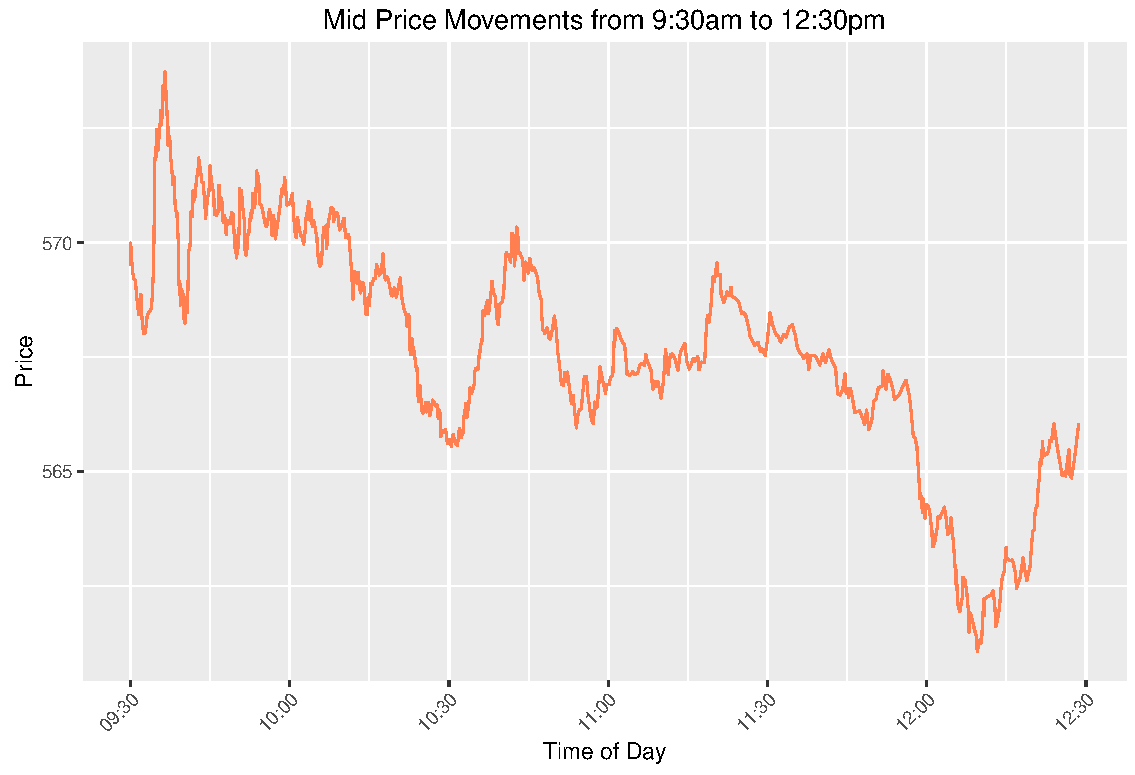
\includegraphics[width=0.8\textwidth]{Mid_Price}
  \caption{Mid Price Movements}
  \label{fig:find6}
\end{figure}

\section{Conclusion}
It is an inherent assumption in the trading industry that future stock movements are guided by historical data. However, after considering several machine learning and statistical models, we found that it is incredibly difficult to predict price movements due to the volatile nature of the stock market. While model accuracies were generally only around 60\%, we suggest that financial agencies implement the random forest model. In our analysis, the random forest produced the highest accuracy and outperformed both the SVM and logistic regression models. This may be partially explained by the randomness associated with the model. Additionally, we found that a passive trading strategy tends to decrease losses in comparison to active strategies when predictions are less than accurate. Machine learning techniques have only recently been incorporated into stock market predictions. While they have the potential to benefit investors, they are still controversial and have much room for growth. 


\bibliographystyle{plain}
\bibliography{finance}
\begin{thebibliography}{9}

\bibitem{ky} 
Alec N. Kercheval, Yuan Zhang. Modeling High-frequency Limit Order Book Dynamics with Support Vector Machines.
\textit{Quantitative Finance}, 15(8):1315–1329, 2015.

\end{thebibliography}


\end{document}
